\documentclass{article}

\usepackage{amsthm}
\usepackage{tikz}
\usetikzlibrary{shapes,positioning,arrows}
\newcommand{\defined}[1]{{\bf #1}}
\newcommand{\var}[1]{{\em #1}}

\theoremstyle{definition}
\newtheorem{definition}{Definition}

\theoremstyle{remark}
\newtheorem{remark}{Bemerkung}
\begin{document}

\section{Grundlagen}
\begin{definition}
Anwender, aktiver Anwender\\
Die Benutzer des Programmes werden im folgenden als \defined{Anwender} bezeichnet.
  Im Folgendenden bezeichnen \var{A}, \var{B} zwei Anwender, die das Programm 
verwenden.\\
  Aus technischen Gr\"unden wird einer der beiden Anwender als 
\defined{aktiver Anwender} bezeichnet und der andere der beiden Anwender als
\defined{passiver Anwender}. Der aktive Anwender ist in der Lage, den Ablauf
eines Protokolles zu initiieren, w\"ahrend der passive Anwender auf die 
Initiierung eines Protokolles durch den aktiven Anwender wartet. Es sei im
folgenden \var{A} der aktive Anwender und \var{B} der passive Anwender.
\end{definition}

\begin{definition}
Wissen, Wissen eines Anwenders, gemeinsames Wissen.\\
Wenn \var{A} ein Anwender ist, so bezeichnen Ausdr\"ucke der Form 
\defined{\var{A.x}} f\"ur Variablen \var{x} \defined{Wissen des Anwenders}. 
Auf das Wissen des Anwenders kann nur der Anwender selbst zugreifen.
Das Wissen eines Anwenders kann \defined{\var{A.x} = \var{e}} erweitert werden.\\
Wenn ein Ausdruck \var{e} als \defined{gemeinsames Wissen c} bezeichnet wird, 
so ist dies \"aquivalent dazu, dass f\"ur alle beteiligten Anwender 
A \var{A.c} = \var{e} ist.
\end{definition}

\begin{definition}
Protokoll.\\
Wir bezeichnen im Folgenden eine Sequenz von Nachrichtenaustauschen zwischen
zwei Anwendern als \defined{Protokoll}
\end{definition}

\begin{definition}
Zwei-Parteien-Berechnung, private Zwei-Parteien-Berechnung, Eingabe, Ausgabe\\
Gegeben zwei Anwender \var{A}, \var{B} mit Wissen \var{A.i} und \var{B.i}
und eine Funktion \var{f}, dann wird ein Protokoll als
\defined{Zwei-Parteien-Berechnung} von Wissen j bezeichnet, wenn nach 
Ausf\"uhrung des Protokolls  \(A.j = f(A.i, B.i) \wedge B.j = f(A.i, B.i) \)
gilt. Wir bezeichnen i als \defined{Eingabe} des Protokolles der Anwender
und j als \defined{Ausgabe} des Protokolles.\\
Wenn ausserdem gilt, dass \var{A} nur \var{A.j} als Wissen ueber \var{B.i}
erh\"alt und dass \var{B} nur \var{B.j} als Wissen ueber \var{A.i} erh\"alt,
dann bezeichnen wir das Zwei-Parteien-Protokoll als \defined{privates
Zwei-Parteien-Protokoll}.
\end{definition}

\begin{remark}
Wenn ein Zwei-Parteien-Protokoll eine Funktion \var{f} berechnen soll,
die Eingaben \var{X} zus\"atzlich zum Wissen der Benutzer erfordert, 
kann dies durch Definition einer Funktion \var{f'(i, j) = f(x, i, j)}
erreicht werden. Dadurch k\"onnen beispielsweise gemeinsames Wissen oder
zuvor festzulegende Parameter genutzt werden. Damit ist die Definition 4
ausreichend, um beliebige Funktionen zu beschreiben.
\end{remark}

\begin{definition}
Phase, private Phase\\
Wir bezeichnen im Folgenden einen Schritt der Anwendung als \defined{Phase}.
Eine Phase erfordert ein gewisses \defined{Vorwissen} der beteiligten Anwender
und garantiert dann, dass nach Ausfuehren der Phase ein gewisses anderes
Wissen erlangt wird. Rein technisch ist eine Phase also nur ein Synonym f\"ur 
eine Funktion auf dem Wissen der Anwender. Damit ergibt sich jedoch, dass
sich auch die Phasen klassifizieren lassen. Eine \defined{private Phase} ist
somit eine Phase, bei der die beteiligten Anwender \"uber das Vorwissen der
anderen beteiligten Anwender nur das Wissen erhalten, dass sie aus dem 
durch die Phase berechneten Wissen schlussfolgern k\"onnen. Eine
\defined{getrennte Phase} ist eine Phase, welche keine Kommunikation zwischen
den Anwendern erfordert.\\
Im folgenden werden wir Bilder von Phasen darstellen. In diesen Bildern werden
im Allgemeinen nur zwei Anwender dargestellt sein. In diesem Bild ist das
Vorwissen und das erhaltene Wissen der Anwender als Rechtecke dargestellt
werden. Das Wissen der Anwender ist durch eine vertikale Linie getrennt und 
der linke Anwender wird ,,Alice'' genannt, w\"ahrend der rechte Anwender Bob
genannt wird. Die Ausf\"uhrung einer Phase wird als Kreis zwischen beiden 
Anwendern dargestellt werden, Pfeile von einem Wissens-Rechteck in 
einen solchen Phasen-Kreis sollen andeuten, dass die Phase dieses Wissen
verwendet und Pfeile von einem solchen Phasen-Kreis zu einem Wissensrechteck
sollen andeuten, dass die Phase dieses Wissen erzeugt. Falls eine Phase 
getrennt ist, wird der bzw die Phasenkreise vollst\"andig in die H\"alfte eines
Anwenders gezeichnet, andernfalls wird der Phasenkreis auf der gestrichelten
Trennlinie gezeichnet werden. Eine einfache \"Ubertragung von Wissen wird
dargestellt als Pfeil von einem Wissens-Recheckt \"uber die gestrichelte
Linie zu einem anderen Wissens-Rechteck. (vgl auch Figure ~\ref{fig:phaseExample})
\end{definition}

\begin{figure}
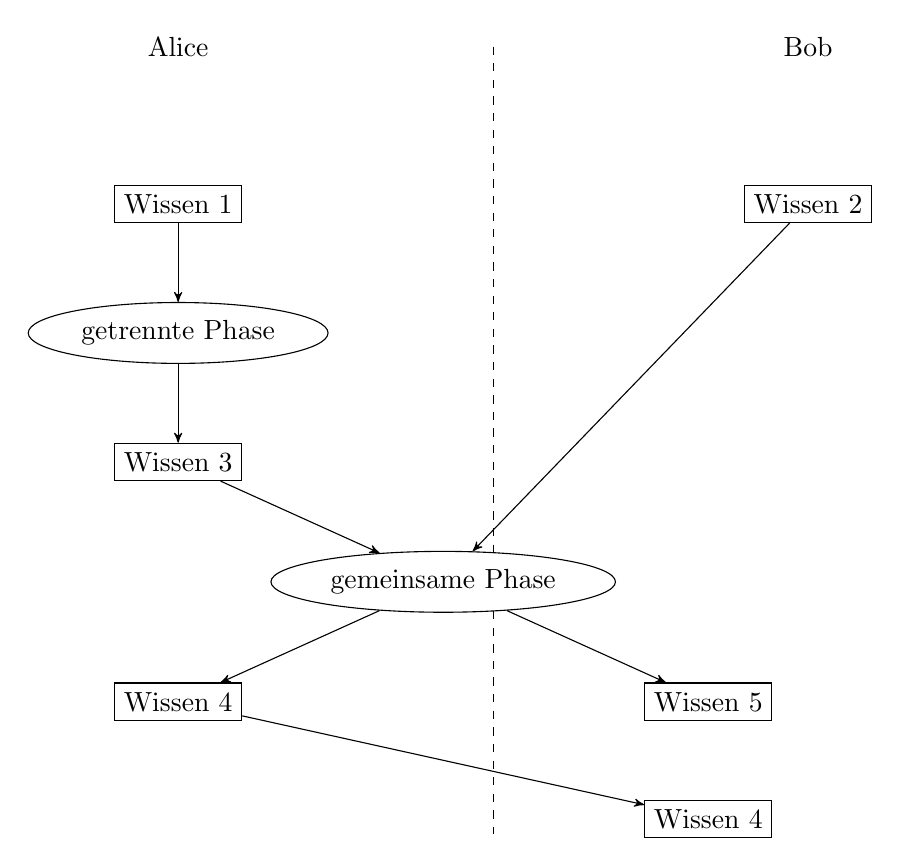
\begin{tikzpicture}
[>=stealth',
 wissen/.style={shape=rectangle,draw},
 phase/.style={shape=ellipse,draw,fill=white}]
\draw (0, 0) node {Alice};
\draw (8, 0) node {Bob};
\draw[dashed] (4, 0) -- (4, -10);
\node (w1) at (0, -2) [wissen] {Wissen 1};
\node (w2) at (8, -2) [wissen] {Wissen 2};
\node[phase] (p1) [below=of w1] {getrennte Phase};
\node[wissen] (w3) [below=of p1] {Wissen 3};
\node[phase] (p2) [below right=of w3] {gemeinsame Phase};
\node[wissen] (w4) [below left=of p2] {Wissen 4};
\node[wissen] (w5) [below right=of p2] {Wissen 5};
\node[wissen] (w6) [below=of w5] {Wissen 4};
\draw[->] (w1) -- (p1);
\draw[->] (p1) -- (w3);
\draw[->] (w3) -- (p2);
\draw[->] (w2) -- (p2);
\draw[->] (p2) -- (w4);
\draw[->] (p2) -- (w5);
\draw[->] (w4) -- (w6);
\end{tikzpicture}
\caption{Phasenbild: Alice mit Phase alleine, beide mit gemeinsamer Phase, Alice sendet Wissen an Bob.}
\label{fig:phaseExample}
\end{figure}
\section{Design der Anwendung}
Es wird nun die Anwendung designed. Hierzu wird r\"uckw\"arts vorgegangen, d.h.,
wir betrachten zuerst, welche Ausgabe die Anwendung produzieren soll und 
betrachten dann Alternativen, diese Ausgabe zu erzeugen. Dadurch ergeben sich
dann weitere ben\"otigte Eingaben f\"ur diese Schlussphase der Anwendung, die
dann rekursiv behandelt werden k\"onnen, bis als Eingabe nur noch die 
vorklassifizierten E-Mails und andere Anwendereingaben \"ubrig bleiben.
An diesem Punkt ist die Anwendung dann fertig designed.\\
Um zu rekapitulieren, die Vision der Anwendung ist:,,Ich habe eine Menge von
vorklassifizierten E-Mails und kenne einen Anwender, der ebenfalls eine Menge
von vorklassifizierten E-Mails hat und will gemeinsam mit diesem einen 
Klassifikator fuer Spam und Nicht-Spam berechnen. Dabei will ich jedoch, dass
er \"uber meine E-Mails nur soviel lernt, wie ich will und wie der Klassifikator
preisgibt.''.
\end{document}
